\documentclass{article}
\usepackage{url,graphicx,color}

\newcommand{\BEASTVersion}{2.2}
\newcommand{\TracerVersion}{1.6}
\newcommand{\FigTreeVersion}{1.4.2}


\def\beast-geo{GEO\_SPHERE}
\def\lt{\textless}
\def\gt{\textgreater}


\begin{document}
    \title{Spherical Phylogeography with BEAST \BEASTVersion}
\author{Remco Bouckaert \url{r.bouckaert@auckland.ac.nz}}
\maketitle

\section{Introduction}


In this tutorial we describe a full Bayesian framework for phylogeography as described in  \cite{sphericalgeo}.
 
You will need the following software at your disposal:

\begin{itemize}

\item {\bf BEAST} - this package contains the BEAST program, BEAUti, TreeAnnotator and other utility programs. This tutorial is written for BEAST v{\BEASTVersion}. It is available for download from \\* \texttt{http://beast2.org/}.
\item {\bf Tracer} - this program is used to explore the output of BEAST (and other Bayesian MCMC programs). It graphically and
quantitively summarizes the distributions of continuous parameters and provides diagnostic information. At the time of
writing, the current version is v{\TracerVersion}. It is available for download from \texttt{http://beast.bio.ed.ac.uk/}.
%\item {\bf FigTree} - this is an application for displaying and printing molecular phylogenies, in particular those obtained using
%BEAST. At the time of writing, the current version is v{\FigTreeVersion}. It is available for download from \texttt{http://tree.bio.ed.ac.uk/}.
\item {\bf Spread} for summarysing the geographic spread in a KML file (available from \url{http://www.kuleuven.ac.be/aidslab/phylogeography/SPREAD.html}.
\item {\bf google-earth} for displaying the KML file (just google for it, if you have not already have it installed).
\end{itemize}


This tutorial guides you through a continuous phylogegraphy analysis of a Hepatitis B Virus (HBV) throughout Eurasia and Africa. The data is described in \cite{sphericalgeo}, but only a subset is used in order to let the analysis run in a short time. The alignment consists of 17 sequences of  3221 characters.

We go through the following steps:
\begin{itemize}
\item The first step is to install the \beast-geo{} package that contains the phylogegraphic model. 
\item Then, we use BEAUti to set up the analysis, and write it to an XML file.
\item We use BEAST to run the MCMC analysis based on the XML file.
\item The results will need to be checked for convergence using Tracer.
\item Finally, we post-process the output of the MCMC so we can visualise the geographical dispersion.
\end{itemize}

\subsection*{Install \beast-geo\ package}

Phylogeography as described in this tutorial is part of the {\tt \beast-geo} package.
If you not already have it installed, you can install the package through BEAUti. Start BEAUti by double clicking on its icon. 
Select the File/Manage packages menu. A dialog pops up showing the packages already installed. 

\begin{center}
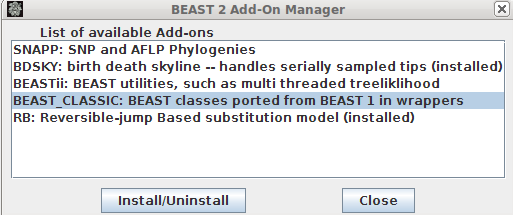
\includegraphics[scale=0.4]{figures/addonmgr.png}
\end{center}

Select the \beast-geo{} entry in the list, and click the Install button. After a little while the dialog is updated and it shows that the package is now installed.

\subsection*{BEAUti}


\subsubsection*{Loading the NEXUS file }

To load a NEXUS format alignment, simply select the \texttt{Import Alignment} option from the File menu. A dialog allows you to choose the kind of data to import, select "Add alignment"

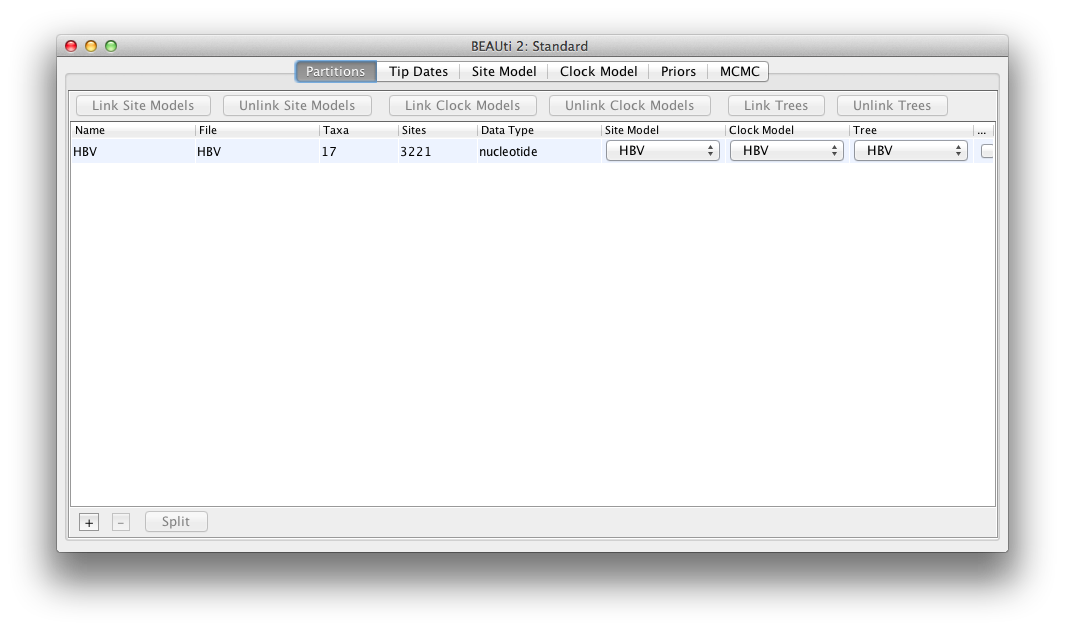
\includegraphics[scale=0.4]{figures/BEAUti_DataPartitions}

Select the file called \texttt{HBV.nex}, which is located in the place where the \beast-geo{} package is installed 
under the {\tt examples/nexus} directory. Typically, packages are installed in different places, depending on your operating system:
\begin{itemize}
\item for Windows, in your home directory (e.g. {\tt c:$\backslash$Users$\backslash$joe}) under the {\tt BEAST} directory,
\item for Mac, in the {\tt Library/Application Support/BEAST} directory in your home directory (e.g. {\tt /Users/joe}),
\item for Linux, in the {\tt .beast} directory in your home directory (e.g {\tt /home/joe}).
\end{itemize}
The file contains an alignment of sequences. The \texttt{HBV.nex} looks like this (content has been truncated):

\begin{verbatim}
#NEXSUS
BEGIN DATA;
       DIMENSIONS  NTAX =17 NCHAR=3224;
       FORMAT DATATYPE = DNA GAP = - MISSING = ?;
       MATRIX   
AB033550_1988_33.3431887795_134.9307404236		CTCCACCACATTCCACCAAGCTCTGCTAGATCCCAGAGTGAGGGGCCTATATTT
AB033554_1985_-2.3045941592_118.5275669247		CTCCACCACGTTCCACCAAACTCTTCAAGATCCCAGAGTCAGGGCTCTGTACTT
AB111946_1998_15.880672531_106.7863444469		CTCAAGCACATTCCACCAAGCTCTGCTAGATCCCAAAGTGAGGGGCCTATACCT
;
END;
\end{verbatim}

\medskip{}

Once loaded, a partition is displayed in the main panel.
You can double click any alignment (partition) to show its detail.

\begin{figure}
\begin{center}

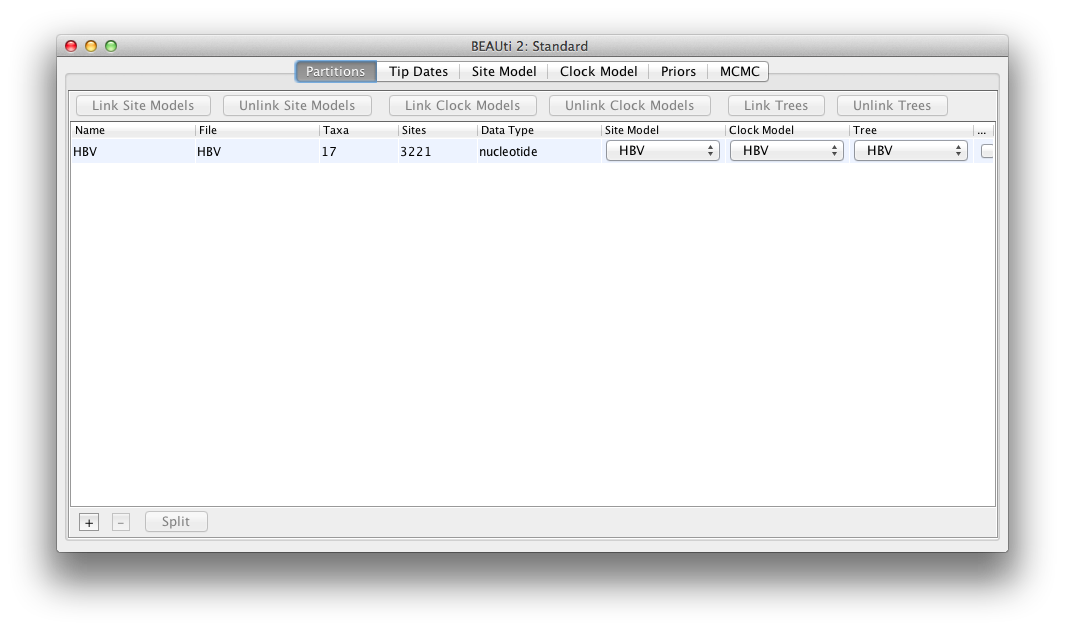
\includegraphics[scale=0.4]{figures/BEAUti_DataPartitions}

\end{center}
\caption{\label{fig.datapartition} Data partition panel after loading alignment.}
\end{figure}

\subsubsection*{Set up dates}

We want to use tip dates for this analysis.

Select the 'Tip Dates' tab, and click the 'Use tip dates' check box.

Since we can derive the date from the taxon names, click the 'Guess' button.

A dialog pops up, where we can specify the dates as follows: the dates are encoded between underscores in the name, and it is the second part. So, we want to split on character (select this box) and take group 2. It should now look like this:

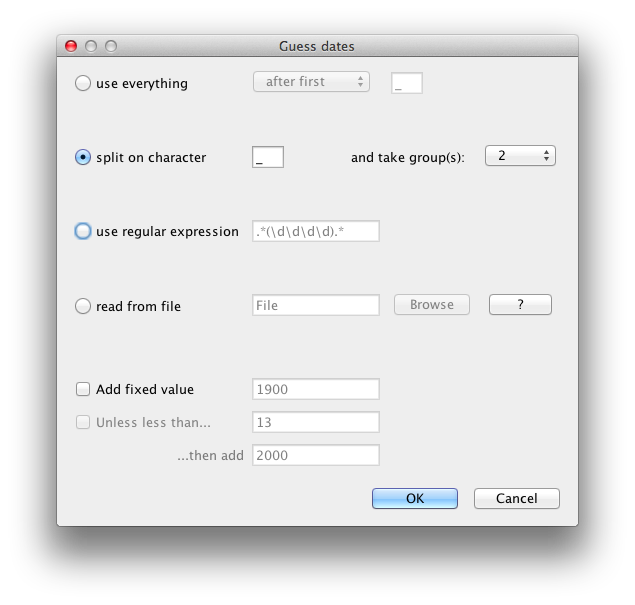
\includegraphics[scale=0.4]{figures/BEAUti_dates.png}

Click OK and the dates are populated by the correct value. Always double check that this happened correctly and no strange outliers or wrong encodings cause any problems, of course.

\subsubsection*{Setting the substitution model}

Select the Site model tab, and change the site model to HKY, and frequency model to `empirical'.
The screen should look like this:

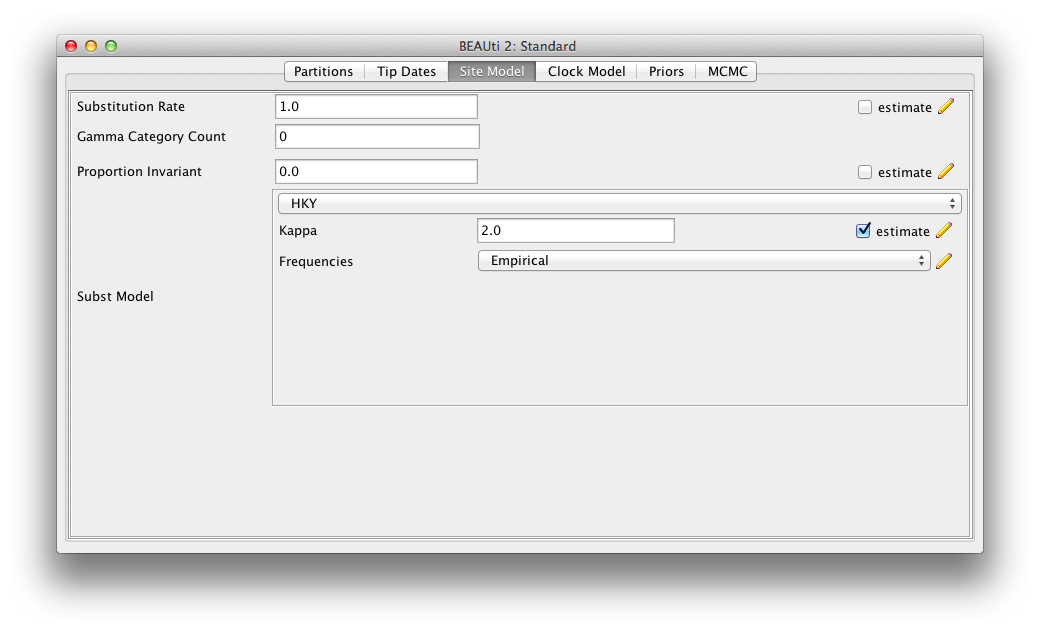
\includegraphics[scale=0.4,clip=true,trim=0 300 0 0]{figures/BEAUti_sitemodel.png}

\subsubsection*{Setting the clock model}

We use a strict clock, so leave the clock tab.

\subsubsection*{Priors and Operators}

Change the tree prior from Yule to Coalescent with Constant Population. The other priors are fine. The screen should look like this:

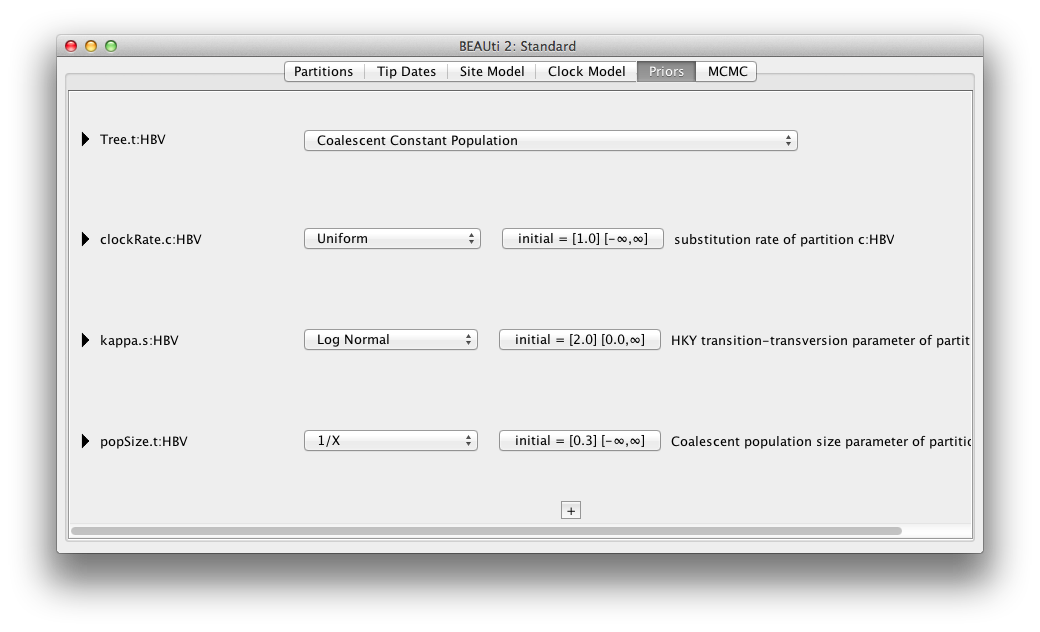
\includegraphics[scale=0.4,clip=true,trim=0 400 0 0]{figures/BEAUti_priors.png}


\subsubsection*{Setting up the geographic model}

Go to the data partitions tab, and click the '+' button at the bottom of the screen.
A dialog pops up where you can select what you want to add. Choose `Add Spherical Geography'
and click `OK'.

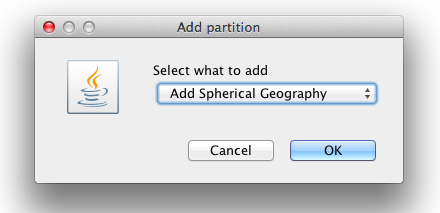
\includegraphics[scale=0.4]{figures/BEAUti_geography1.png}

A new window pops up where you can choose the tree where you want to add geography.
Also, you can change the trait name to `geo';

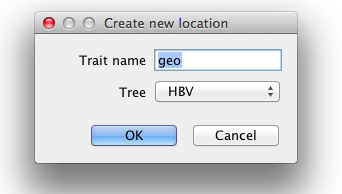
\includegraphics[scale=0.4]{figures/BEAUti_geography2.png}

When you click OK, a dialog is shown where you can enter latitude and longitude for each taxon.
In this tutorial, this information is encoded in the taxon name, so we can guess it from the name. 

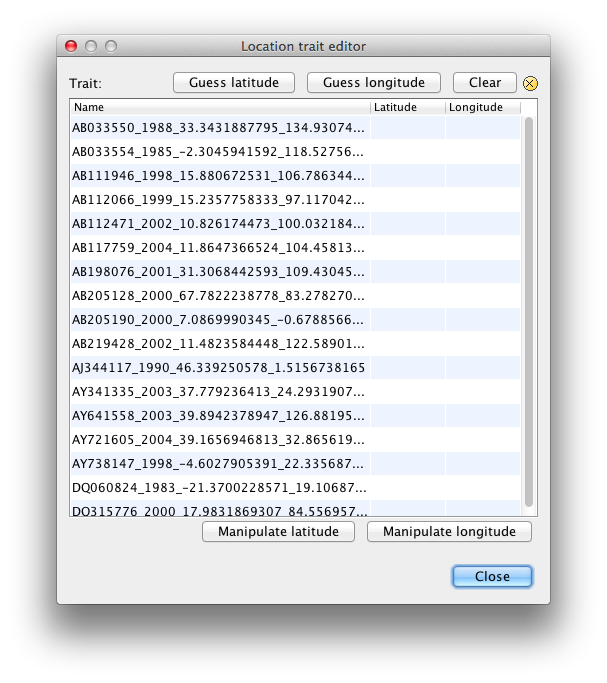
\includegraphics[scale=0.4]{figures/BEAUti_geography3.png}

Click `Guess latitude', and a dialog is shown. Choose `split on character' and take group 3 for the latitude.
When you click OK, the latitude field of the table is populated.

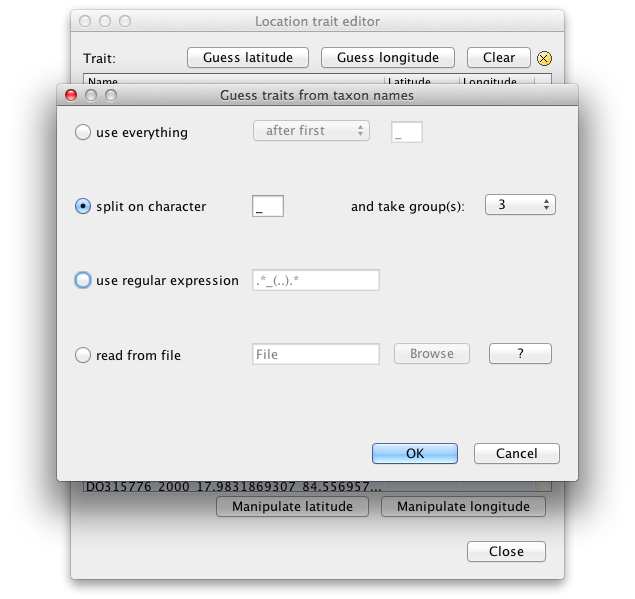
\includegraphics[scale=0.4]{figures/BEAUti_geography4.png}

Click `Guess longitude', and again a dialog is shown. Choose `split on character' and take group 4 for the longitude.

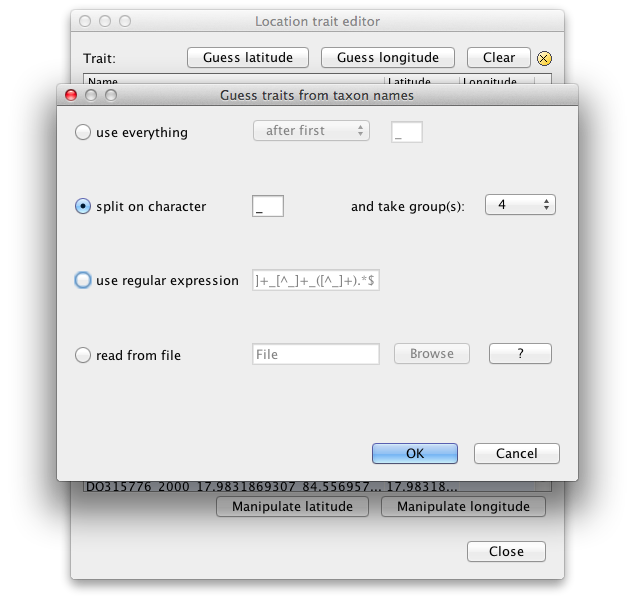
\includegraphics[scale=0.4]{figures/BEAUti_geography5.png}

When you click OK, the table is completely populated. 

{\bf Note  1}: when you have longitudes on the eastern side of the hemisphere  instead of west you may need to make all longitudes negative. The easiest way to do this is to press the 'Manipulate longitude' button. An optionpane pops up where you can enter a formula that is applied to all longitude values, like so:
Key in, '-\$x', and press OK. 

{\bf Note  2}: instead of encoding location information and dates in the name, you can also create a tab-delimited file containing a column with taxon names and latitude/longitude pairs and import them using the  `read from file' entry in the Guess dialog shown aboce. In the \beast-geo/examples/nexus folder, there are two examples, one for time ({\tt HBV\_dates.dat}) and one with geography info ({\tt HBV\_locations.dat}).

Now, the longitudes and latitudes are properly populated, like so:

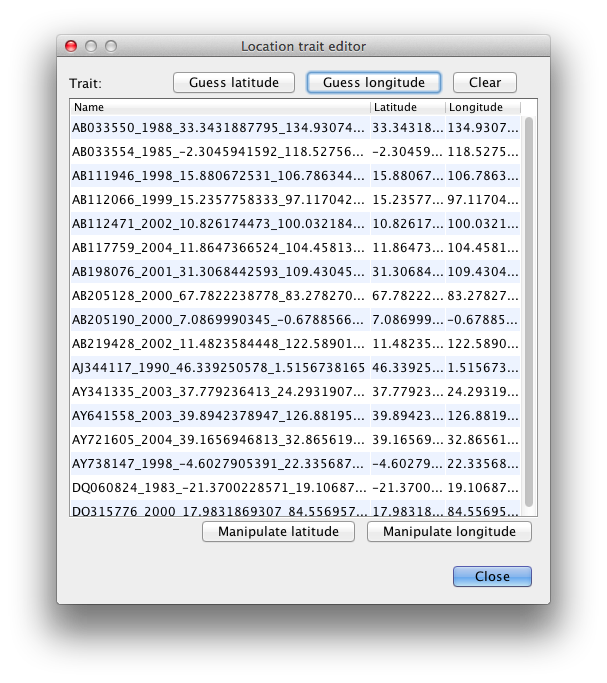
\includegraphics[scale=0.4]{figures/BEAUti_geography6.png}

Click close, and a second data partition is created.

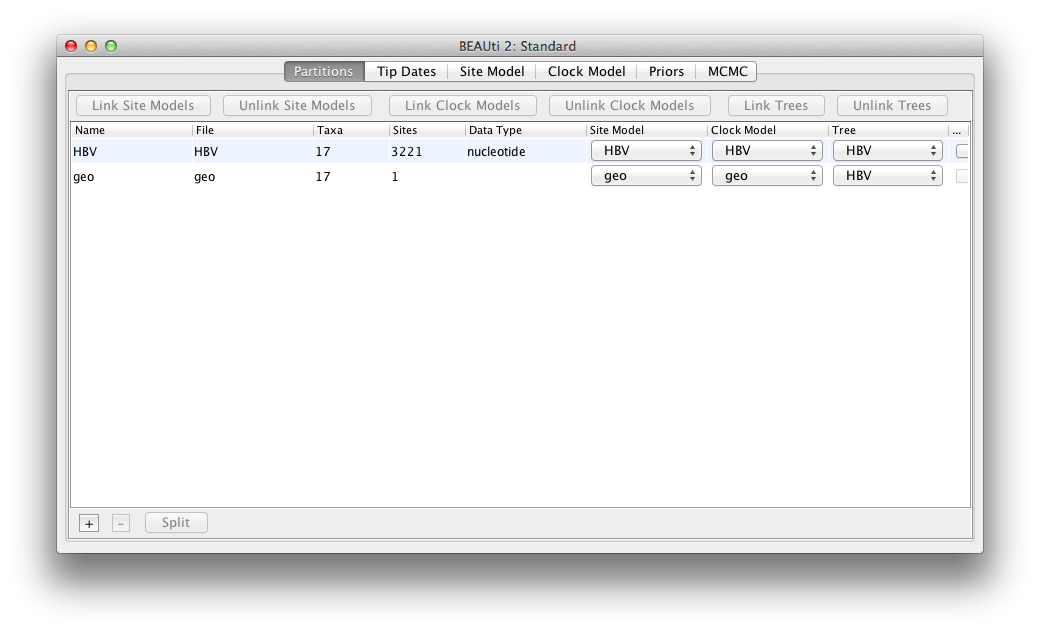
\includegraphics[scale=0.4]{figures/BEAUti_DataPartitions2.png}

The clock model now looks like this:

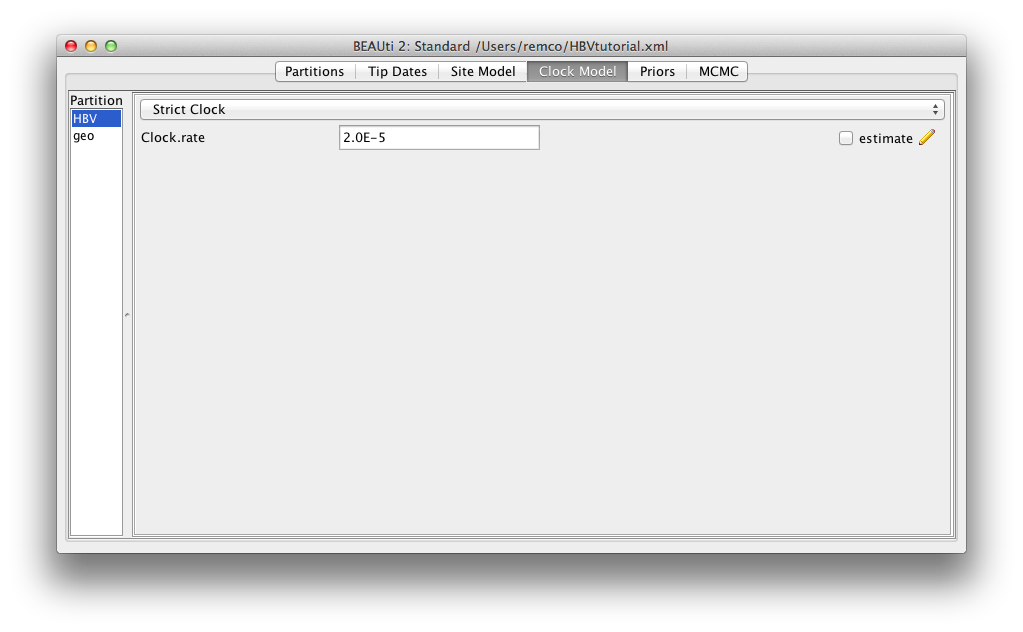
\includegraphics[scale=0.4,clip=true,trim=0 300 0 0]{figures/BEAUti_clockmodel2.png}
In order to speed up convergence, you can set the clock rate to 2e-5 and uncheck the `estimate' checkbox. Initially, it is disabled since by default, whether clock rates are estimated is left to BEAUti. If you uncheck the `Mode/Automatic set clock rates' menu item, you can change the `estimate' checkbox.

For the geography, we select a relaxed clock with log-normal distribution. 

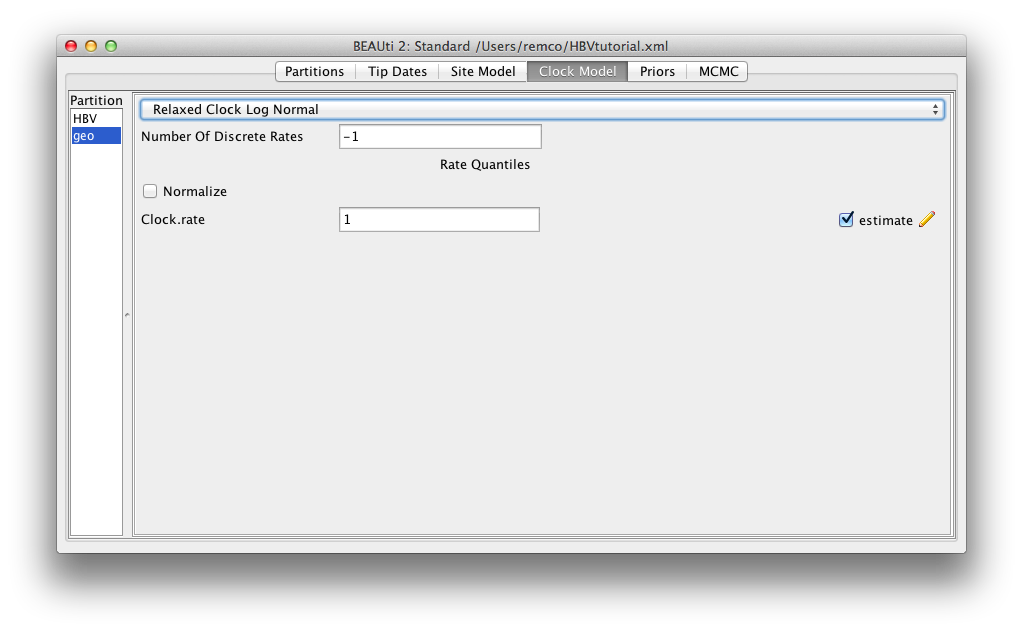
\includegraphics[scale=0.4,clip=true,trim=0 300 0 0]{figures/BEAUti_clockmodel3.png}

The priors now look like this:

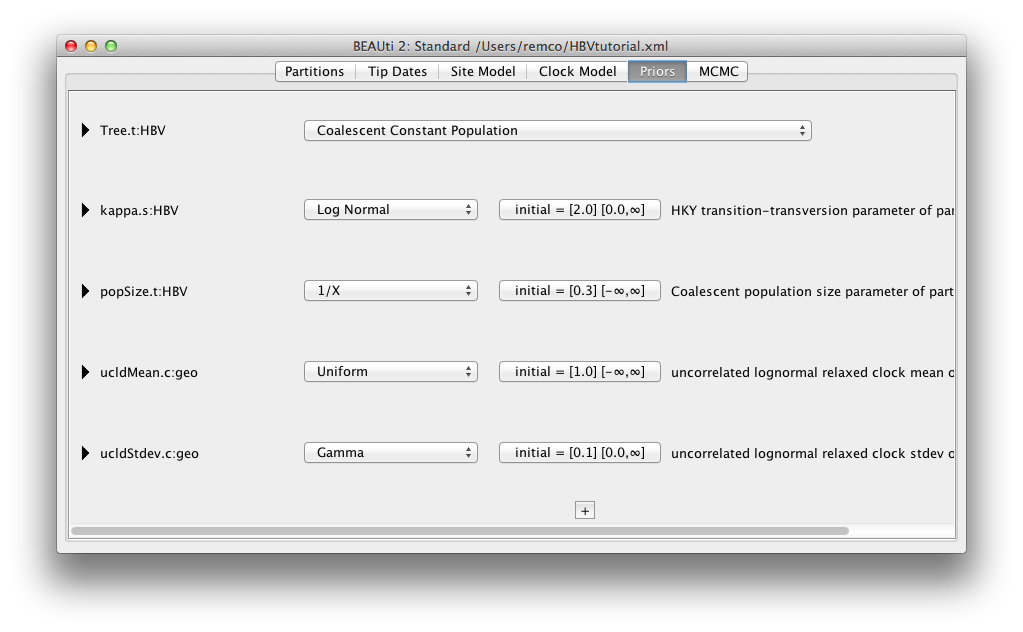
\includegraphics[scale=0.4]{figures/BEAUti_priors2.png}

To get the location edit dialog back, double click the location partition.


\subsubsection*{Setting the MCMC options }

The next tab, {\bf MCMC}, provides more general
settings to control the length of the MCMC and the file names. 

Firstly we have the \textbf{Length of chain}. This is the number of
steps the MCMC will make in the chain before finishing. The appropriate length of the chain depends on the size of the data set, the complexity of the
model and the accuracy of the answer required. The default value of 10,000,000
is entirely arbitrary and should be adjusted according to the size
of your data set. For this data set let's initially set the chain
length to 1,000,000 as this will run reasonably quickly on most modern
computers (less than 5 minutes).

The next options specify how often the parameter values in the Markov
chain should be displayed on the screen and recorded in the log file.
The screen output is simply for monitoring the programs progress so
can be set to any value (although if set too small, the sheer quantity
of information being displayed on the screen will actually slow the
program down). For the log file, the value should be set relative
to the total length of the chain. Sampling too often will result in
very large files with little extra benefit in terms of the precision
of the analysis. Sample too infrequently and the log file will not
contain much information about the distributions of the parameters. 
You probably want to aim to store no more than 10,000 samples so this should be
set to no less than chain length / 10,000.

For this exercise we will set the screen log to 10000 and leave the file log to 1000. The final two
options give the file names of the log files for the sampled parameters and
the trees. These will be set to a default based on the name of the
imported NEXUS file. 

\begin{figure}
\begin{center}

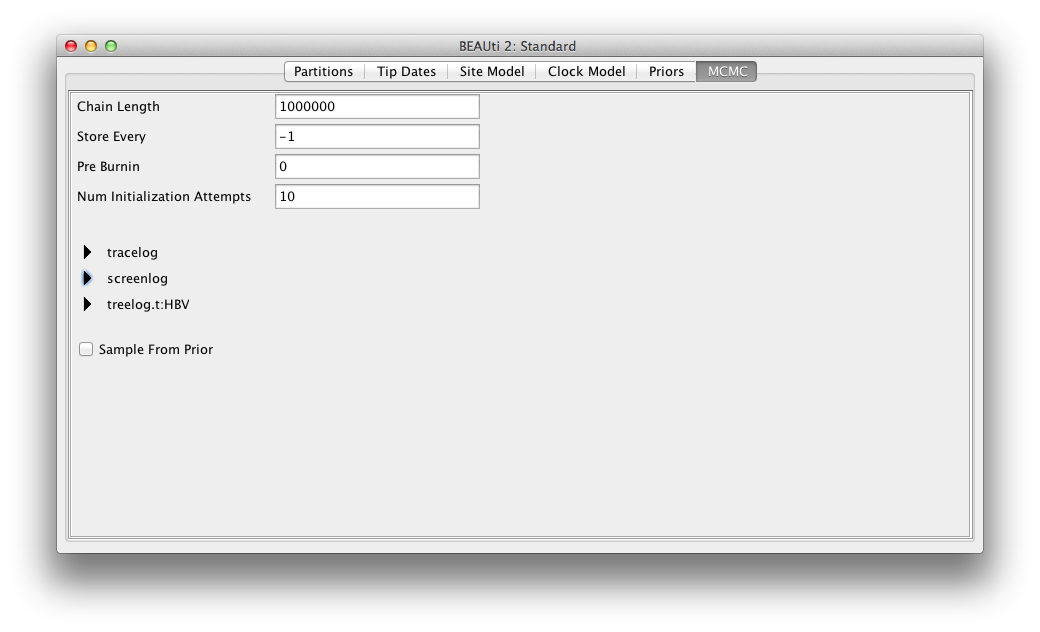
\includegraphics[scale=0.4]{figures/BEAUti_MCMC}

\end{center}
\caption{\label{fig.MCMC} Setting up the MCMC parameters.}
\end{figure}


If you are using windows then we suggest you add the suffix \texttt{.txt} to both of these (so,
\texttt{HBV.log.txt} and \texttt{HBV.trees.txt}) so that Windows recognises
these as text files. 

\subsubsection*{Generating the BEAST XML file }

We are now ready to create the BEAST XML file. To do this, either select the {\bf File/Save} or {\bf File/Save As} option from the \textbf{File} menu. Check the default priors setting and click \textbf{Continue}. Save the file with an appropriate name (we usually end the filename with \texttt{.xml}, i.e., \texttt{HBV.xml}). We are now ready to run the file through BEAST. 

\subsection*{Running BEAST }

Now run BEAST and when it asks for an input file, provide your newly
created XML file as input by click \textbf{Choose File ...}, and then click \textbf{Run}. 

\begin{figure}
\begin{center}

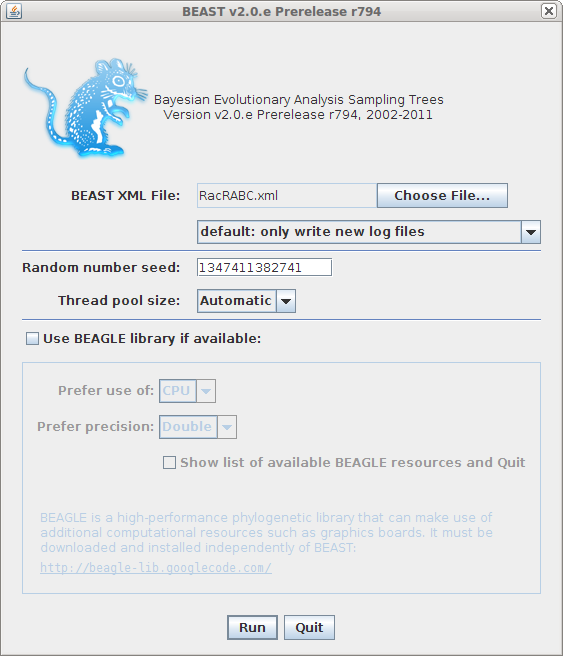
\includegraphics[scale=0.5]{figures/BEAST}

\end{center}
\caption{\label{fig.BEAST} Launching BEAST.}
\end{figure}


BEAST will then run until it has finished
reporting information to the screen. The actual results files are
saved to the disk in the same location as your input file. The output to the screen will
look something like this: 

{\scriptsize   
\begin{verbatim}

                   BEAST v2.2.0 Prerelease, 2002-2014
             Bayesian Evolutionary Analysis Sampling Trees
                       Designed and developed by
 Remco Bouckaert, Alexei J. Drummond, Andrew Rambaut & Marc A. Suchard
                                    
                     Department of Computer Science
                         University of Auckland
                        remco@cs.auckland.ac.nz
                        alexei@cs.auckland.ac.nz
                                    
                   Institute of Evolutionary Biology
                        University of Edinburgh
                           a.rambaut@ed.ac.uk
                                    
                    David Geffen School of Medicine
                 University of California, Los Angeles
                           msuchard@ucla.edu
                                    
                      Downloads, Help & Resources:
                           http://beast2.org/
                                    
  Source code distributed under the GNU Lesser General Public License:
                   http://github.com/CompEvol/beast2
                                    
                           BEAST developers:
   Alex Alekseyenko, Trevor Bedford, Erik Bloomquist, Joseph Heled, 
 Sebastian Hoehna, Denise Kuehnert, Philippe Lemey, Wai Lok Sibon Li, 
Gerton Lunter, Sidney Markowitz, Vladimir Minin, Michael Defoin Platel, 
                 Oliver Pybus, Chieh-Hsi Wu, Walter Xie
                                    
                               Thanks to:
          Roald Forsberg, Beth Shapiro and Korbinian Strimmer

Random number seed: 1418328679458

File: HBVtutorial.xml seed: 1418328679458 threads: 1
Probing: beagle.jar Skip loading file:/Users/remco/workspace/beast2/lib/beagle.jar: contains classs beagle.Beagle that is already loaded
Probing: colt.jar Skip loading file:/Users/remco/workspace/beast2/lib/colt.jar: contains classs cern.clhep.PhysicalConstants that is already loaded
Probing: commons-math3-3.1.1.jar Skip loading file:/Users/remco/workspace/beast2/lib/commons-math3-3.1.1.jar: contains classs org.apache.commons.math3.linear.OpenMapRealVector$OpenMapEntry that is already loaded
Probing: debug-1.0.jar Skip loading file:/Users/remco/workspace/beast2/lib/debug-1.0.jar: contains classs org.jdesktop.swinghelper.debug.CheckThreadViolationRepaintManager$1 that 
...

\end{verbatim}}

\subsection*{Analysing the results}

Run the program called {\bf Tracer} to analyse the output of BEAST. When the main
window has opened, choose {\bf Import Trace File...} from the {\bf File} menu and select the file that
BEAST has created called \texttt{HV.log}.
You should now see a window like in Figure \ref{fig.tracer1}.

\begin{figure}
\begin{center}

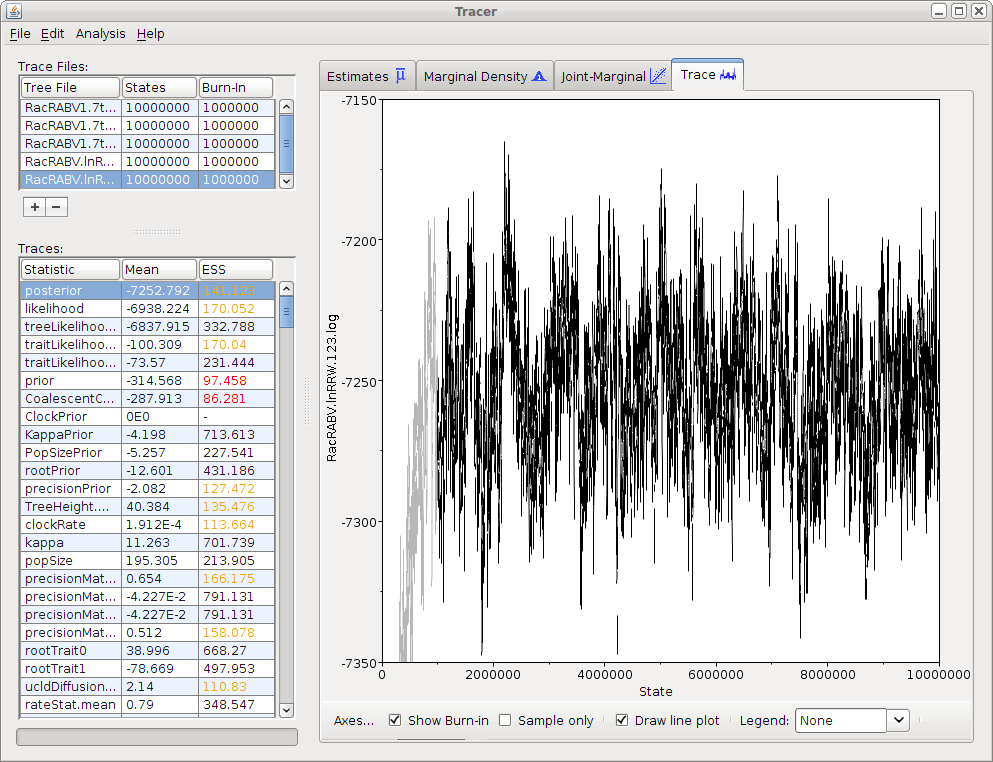
\includegraphics[width=\textwidth]{figures/Tracer}

\end{center}
\caption{\label{fig.tracer1} Tracer with the HBV data.}
\end{figure}


Remember that MCMC is a stochastic algorithm so the actual numbers will not be exactly the same.

On the left hand side is a list of the different quantities that BEAST has logged. There are traces for the posterior (this
is the log of the product of the tree likelihood and the prior probabilities), and the continuous parameters. Selecting a trace
on the left brings up analyses for this trace on the right hand side depending on tab that is selected. When first opened, the
`posterior' trace is selected and various statistics of this trace are shown under the Estimates tab.
In the top right of the window is a table of calculated statistics for the selected trace. 

Tracer will plot a (marginal posterior) distribution for the selected parameter and also give you statistics such as the mean and median. The \texttt{95\% HPD lower} or \texttt {upper} stands for {\it highest posterior density interval} and represents the most compact interval on the selected parameter that contains 95\% of the posterior probability. It can be thought of as a Bayesian analog to a confidence interval. 


\section*{Questions}

To determine whether a relaxed clock is supported by the data over a strict clock,
examine the coefficient of variation. What is the mean, and the shape of the distribution
of the coefficient of variation? Is a relaxed clock is appropriate for this data?

\vspace{5 mm}
\framebox(420,60){}
\vspace{5 mm}



\subsection*{Obtaining an estimate of the phylogenetic tree}

BEAST also produces a sample of plausible trees. 
These can be summarized using the program {\bf TreeAnnotator}. This will take the set of trees and identify a single tree that best represents the posterior distribution. It will then annotate this selected tree topology with the mean ages of all the
nodes as well as the 95\% HPD interval of divergence times for each clade in the selected tree. It will also calculate the posterior clade probability for each
node. Run the {\bf TreeAnnotator} program and set it up to look like in Figure \ref{fig.TreeAnnotator}.

\begin{figure}
\begin{center}

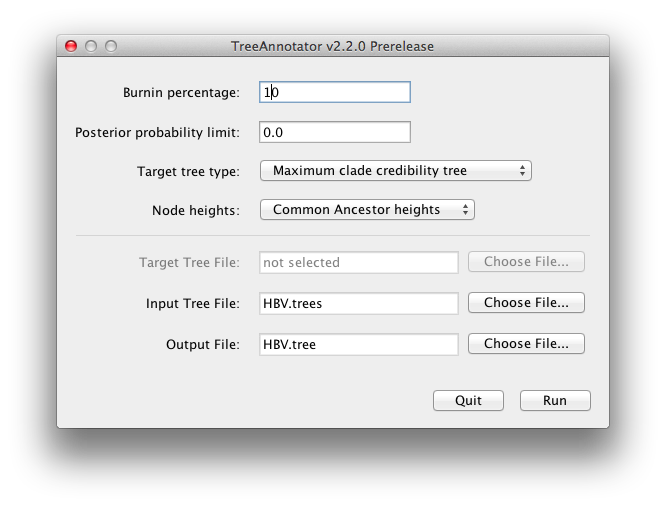
\includegraphics[width=0.75\textwidth]{figures/TreeAnnotator}

\end{center}
\caption{\label{fig.TreeAnnotator} Using TreeAnnotator to summarise the tree set.}
\end{figure}

{\color{red}TODO: what about  TreeAnnotator.processBivariateAttributes?}

The burnin is the number of trees to remove from the start of the sample. Unlike {\bf Tracer} which specifies the number of steps as a burnin, in {\bf TreeAnnotator} you need to specify the actual number of trees. For this run, we use the default setting.

The {\bf Posterior probability limit} option specifies a limit such that if a node is found at less than this frequency in the sample of trees (i.e., has a posterior probability less than this limit), it will not be annotated. The default of 0.5 means that only nodes seen in the majority of trees will be annotated. Set this to zero to annotate all nodes.

For {\bf Target tree type} you can either choose a specific tree from a file or ask TreeAnnotator to find a tree in your sample. The default option, {\bf Maximum clade credibility tree}, finds the tree with the highest product of the posterior probability of all its nodes.

Choose {\bf Mean heights} for node heights. This sets the heights (ages) of each node in the tree to the mean height across the entire sample of trees for that clade.

For the input file, select the trees file that BEAST created (by default this will be called \texttt{HBV.trees}) and select a file for the output (here we called it \texttt{HBV.tree}).

Now press \texttt{Run} and wait for the program to finish.

\subsection*{Viewing the Tree}

\if0
We can look at the tree in another program called {\bf FigTree}. Run this program, and open
the \texttt{HBV.tree} file by using the Open command in the File menu. The tree should appear.
You can now try selecting some of the options in the control panel on the left. Try selecting
{\bf Node Bars} to get node age error bars. Also turn on {\bf Branch Labels} and select {\bf posterior} to get
it to display the posterior probability for each node. Under {\bf Appearance} you can also tell FigTree
to colour the branches by the rate.
You should end up with something like Figure \ref{fig.figtree}.

\begin{figure}
\begin{center}

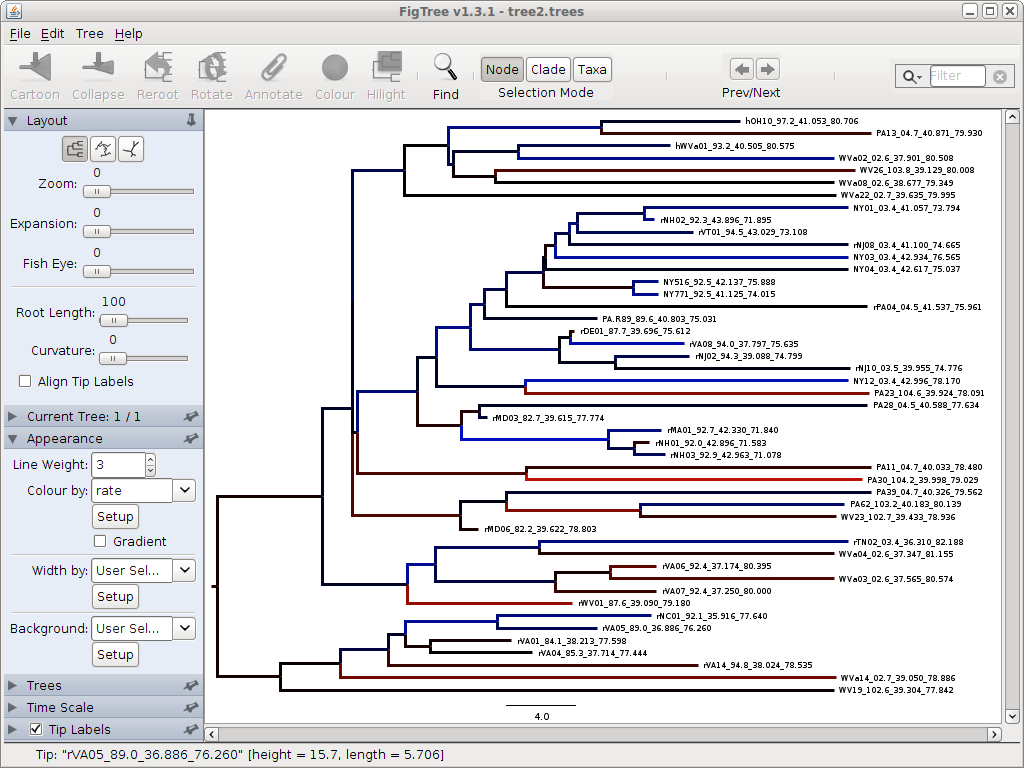
\includegraphics[width=\textwidth]{figures/figtree.png}

\end{center}
\caption{\label{fig.figtree} Figtree representation of the summary tree. Branch colours represent diffusion rates.}
\end{figure}
\fi

We can look at the tree posterior in another program called {\bf DensiTree}.
You can load the tree set (note this is NOT the summary tree, but the complete set) into DensiTree and set it up as follows.

\begin{itemize}
\item Show a root-canal tree to guide the eye. Perhaps, the intensity of the trees is not large enough, so you might want to increase the intensity by clicking the icon in the button bar. If the root canal tree has negative branch lengths, this is an indication that there is little support for the clade under the branch that goes into the wrong direction. You can experiment with a few different root canal trees to solve this problem. Potentially, you need to reorder the taxa (choose something under the Edit/Shuffle submenu) to make the root canal tree look good.
\item Show a grid, and play with the grid options to only show labels in years (revers order, set origin to 2000).
\end{itemize}


The image should look something like Figure \ref{fig.DensiTree}

\begin{figure}
\begin{center}

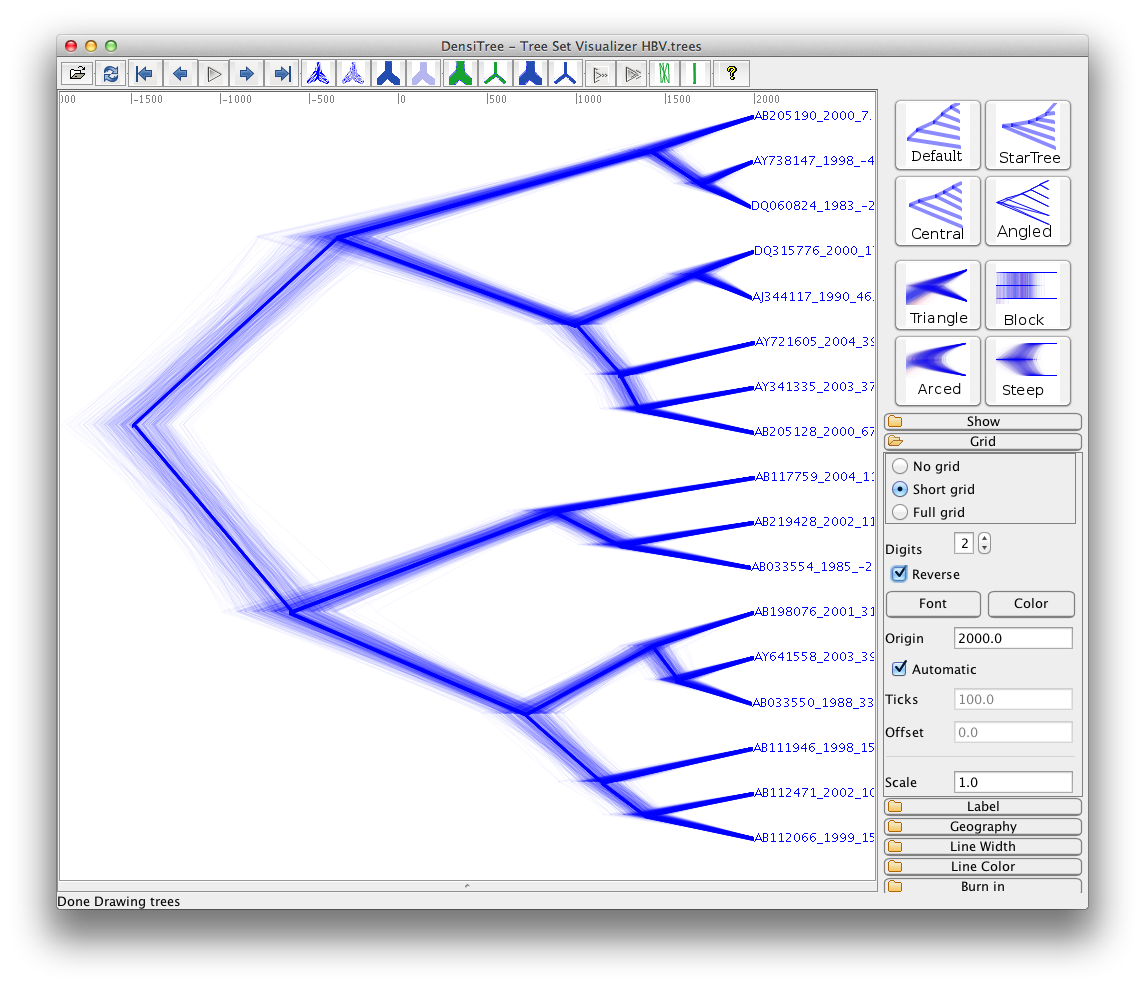
\includegraphics[width=\textwidth]{figures/DensiTree}

\end{center}
\caption{\label{fig.DensiTree} DensiTree representation of the tree.}
\end{figure}

\subsection*{Post processing geography}

Start spread by double clicking the spread.jar file.

Select the 'continuous' tab.

Click the load-button and select the summary tree file.

Select location.geo1 as latitude attribute and location.geo2 as longitude attribute.

Now, open the 'Output' tab in the panel on the left hand side. Here, you can choose where to save the kml file (default {\tt output.kml}).

Click the plot button, and a world map appears with the tree superimposed onto the area where the rabies epidemic occurred.

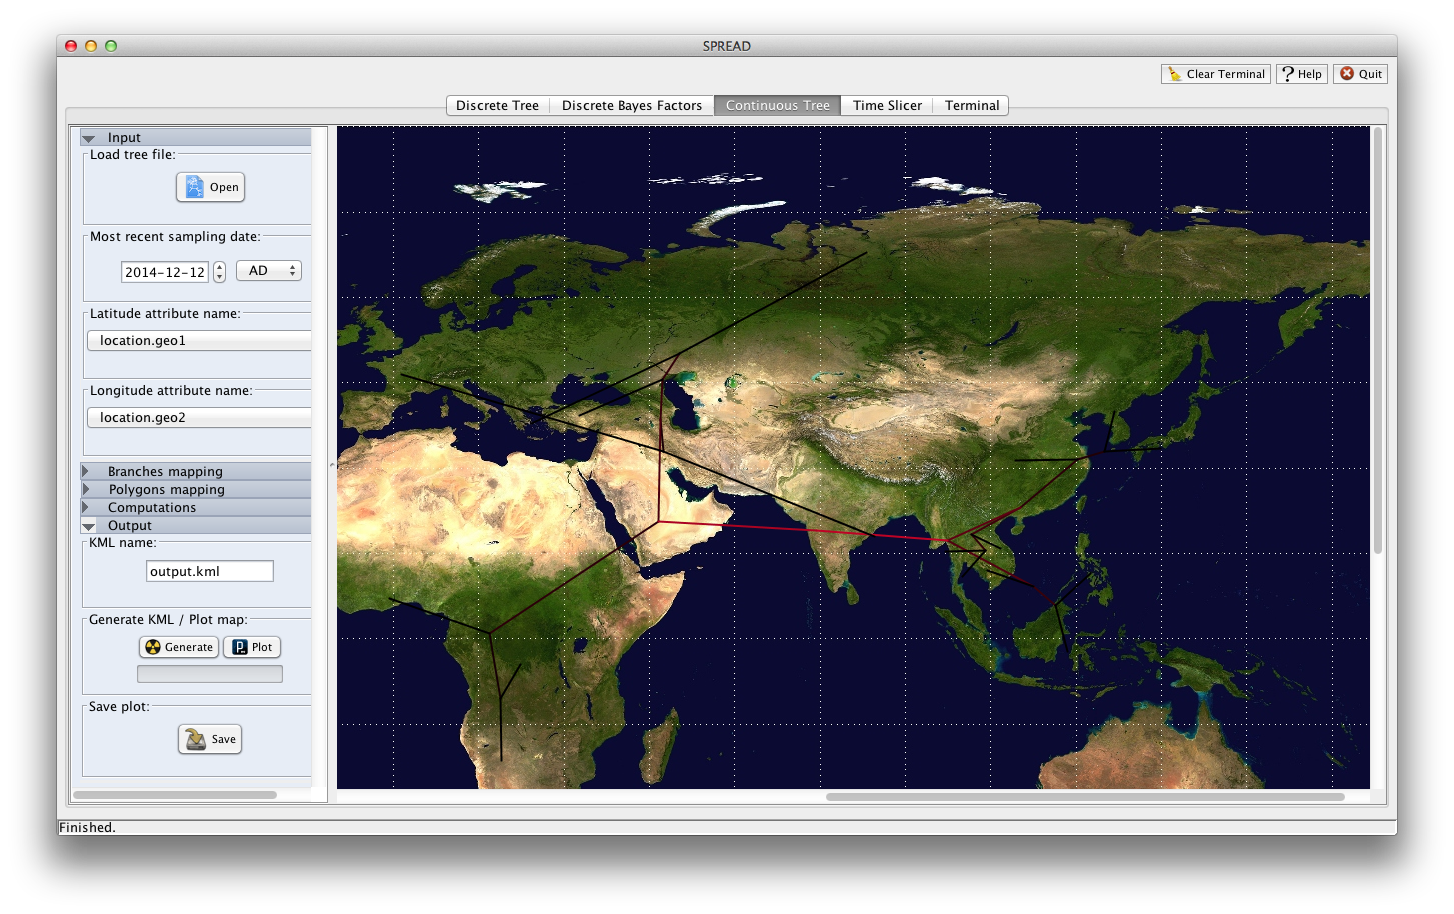
\includegraphics[width=\textwidth]{figures/spread.png}

The KML file can be read into google earth. Here, the spread of the epidemic can be animated through time. The coloured areas represent the 95\% HPD regions of the locations of the internal nodes of the summary tree.

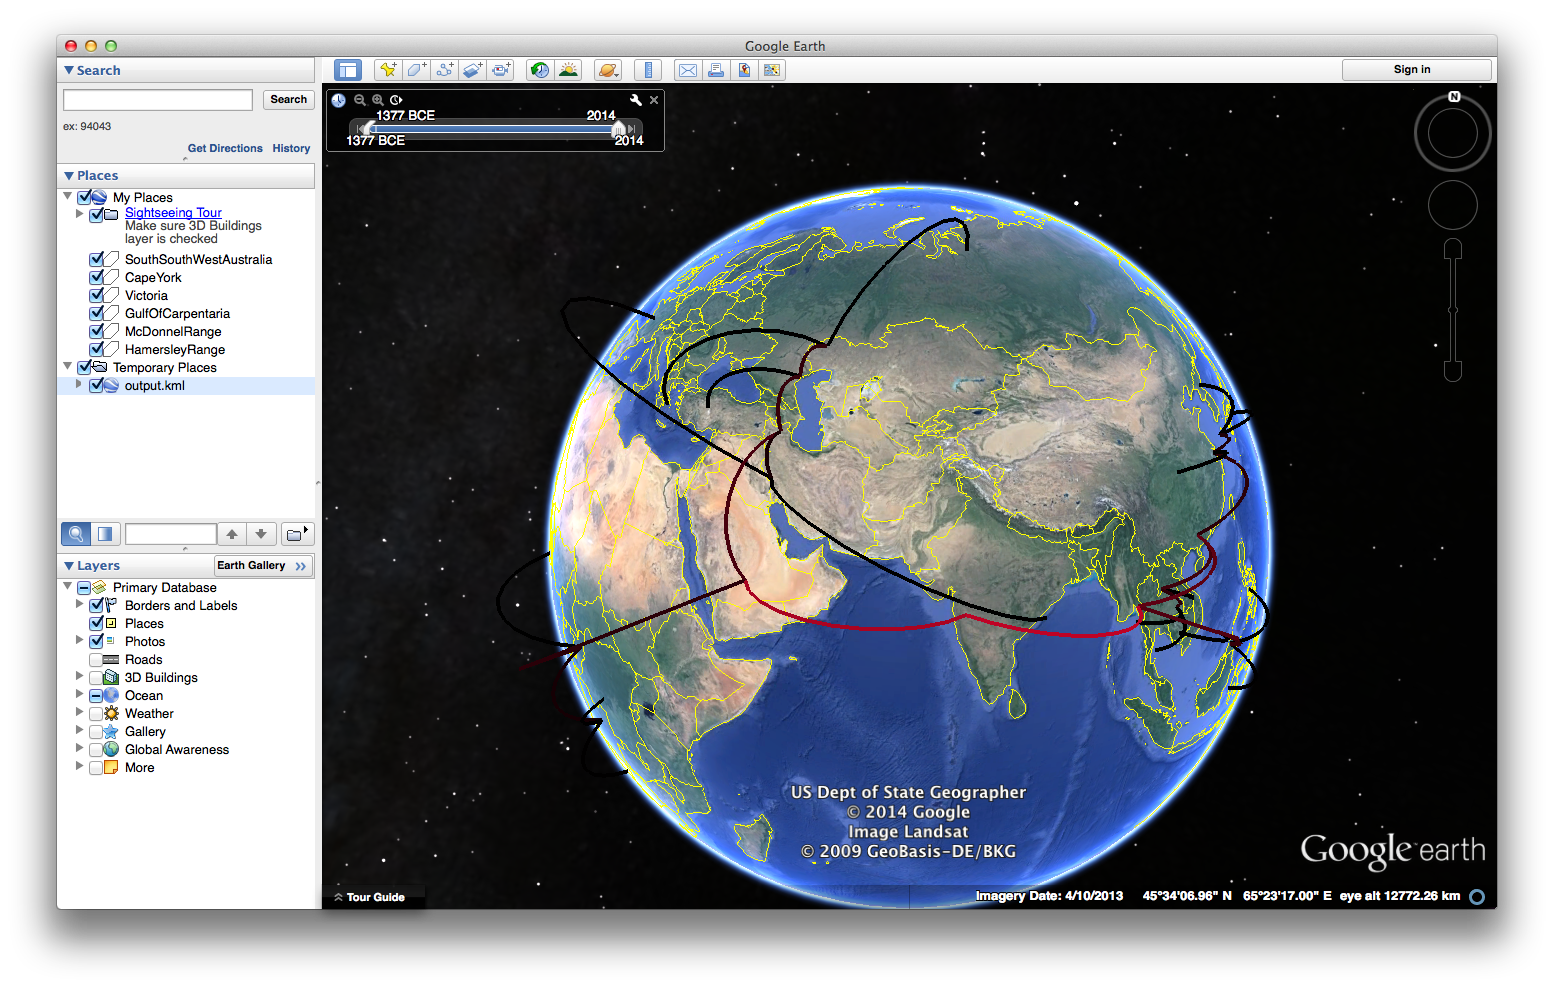
\includegraphics[width=\textwidth]{figures/google-earth.png}


You can use the HeatMapMaker utilty that comes with GEO\_SPHERE to create an image where each dot represents a locati
on of an internal node and the color represents the age. To start HeatMapMaker, start the BEAST-AppStore (double clic
k the AppStore icon in the BEAST-folder), and a window appears like so:

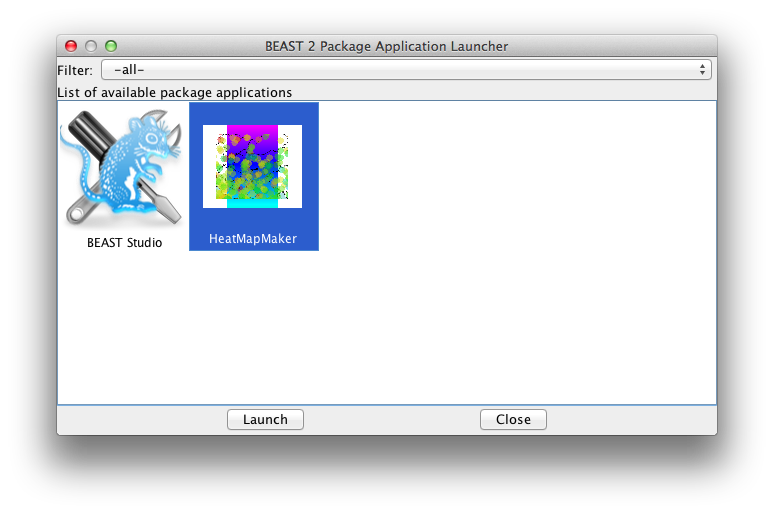
\includegraphics[scale=0.4]{figures/AppStore}

Select HeatMapMaker, then click the launch button and the HeatMapMaker interface appears.

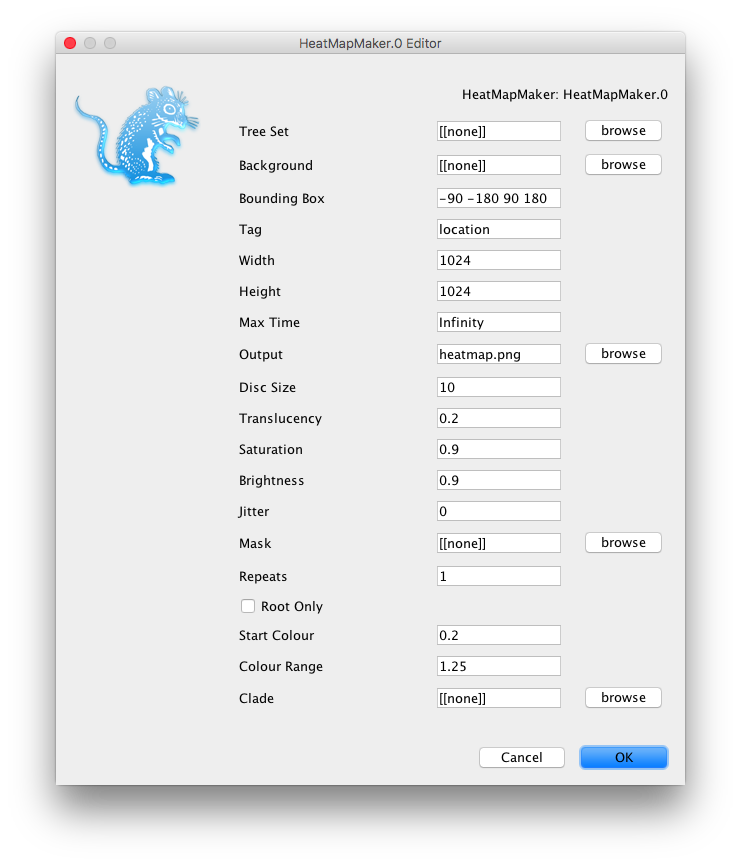
\includegraphics[scale=0.4]{figures/HeatMapMaker}

You can change the following options:

\begin{itemize}
\item tree Set: file containing tree set annotated with locations
\item background: image file with a map for the background
\item bounding Box: bounding box of the background image, default -90 -180 90 180
\item tag: tag used in annotated of locations
\item width: width of the heat map, default 1024
\item height: heightof the heat map, default 1024
\item max Time: maximum time (all older nodes will be coloured red 
\item output: where to save the file, default /tmp/heatmap.png
\item disc Size: size of the dots used to draw heat map
\item translucency: translucency of the dots used to draw heat map (a number between 0=invisible and 1=solid)
\item saturation: saturation of colour for the dots
\item brightness: brightnessof colour for the dots 
\end{itemize}

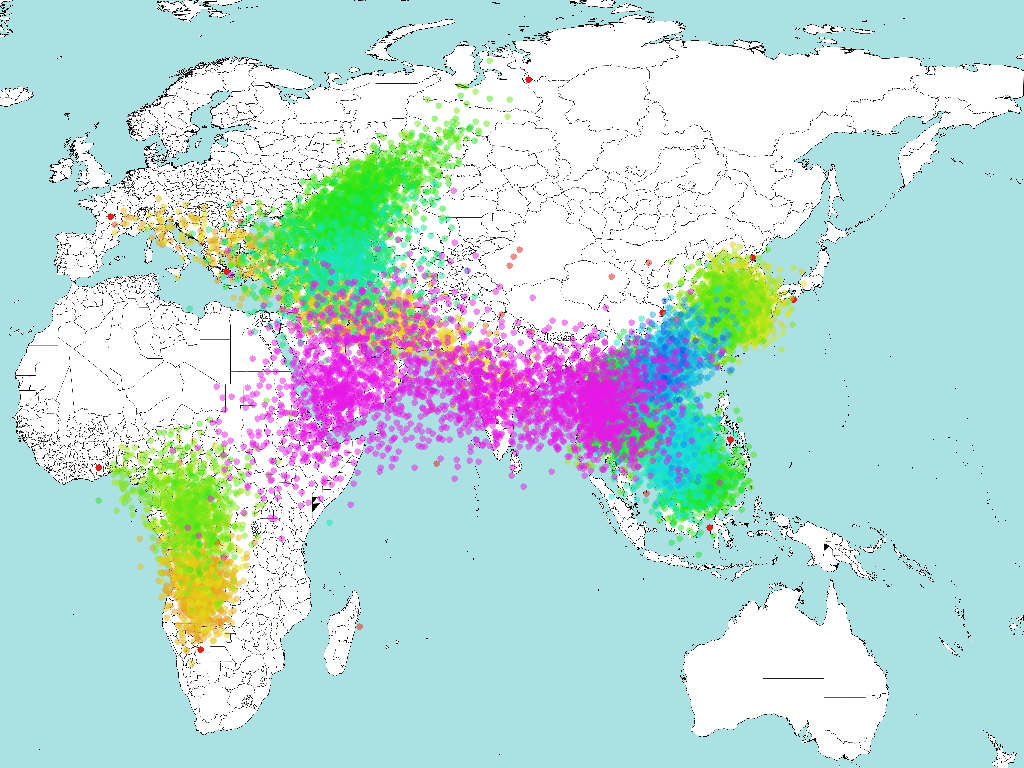
\includegraphics[width=0.8\textwidth]{figures/heatmap}
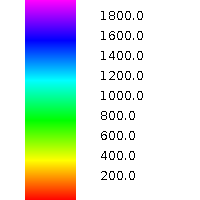
\includegraphics[width=0.19\textwidth]{figures/legend}


\subsection*{Advanced}
\subsubsection*{Sampling tip locations}
At this point in time, there is no BEAUti support to allow sampling of tip locations, but it can be done by editing the XML once it is produced by BEAUti.




First, you need to add an entry to the state, and add operators.
Second, you have to define a set of regions, either by KML or by colouring a bitmap image in Mercatore projection. KML regions can be drawn in google-earth and bitmap images in Mercator projection can be produced using the MapMaker utility that you can start from the BEAST AppStore. Once you created a world map with MapMaker, you can colour in the region you want to sample from.

To set up the state, add the following line (where "geo" is the name used for the geography partition)

\begin{verbatim}
<stateNode idref="location.geo"/>
\end{verbatim}

Next, add a LocationOperator to the set of operators (inside the MCMC element, where the other operators are):

\begin{verbatim}
<operator id='location.sampler' spec='sphericalGeo.LocationOperator' 
    location='@location.geo' 
    likelihood='@slocationtreeLikelihood.geo' weight='30'/>
\end{verbatim}


To specify a KML region, add the following fragment to the XML at the top level (just under the alignment, but above the run element would be a good place).

\begin{verbatim}
<region id='China' spec='sphericalGeo.region.KMLRegion' kml='kml/China.kml'/>
\end{verbatim}

This creates a KMLRegion with id China, and reads in the kml file in the folder kml from file China.kml. To create a bitmap region from a bitmap file stored in say regions/China.png, you can use

\begin{verbatim}
<region id='China' spec='sphericalGeo.region.BitMapRegion'
	file='regions/China.png'/>
\end{verbatim}
There is an extra option to specify a bounding box by two latitude/longitude pairs if the bitmap only covers a small region of the map instead of the whole world:
\begin{verbatim}
<region id='China' spec='sphericalGeo.region.BitMapRegion'
	file='regions/China.png' bbox=''/>
\end{verbatim}



Now we defined a region, suppose you want to sample taxon AF182802 from the region of China, you add

\begin{verbatim}
<geoprior location='@location.geo' tree='@Tree.t:hbv' region='@China'
	spec='sphericalGeo.GeoPrior'>
	<taxon id='AF182802' spec='Taxon'/> 
<geoprior>
\end{verbatim}

inside the element with id="slocationtreeLikelihood.geo" (where 'geo' is the name of the partition for spherical geography, and 'hbv' the name of the partition with the alignment).


If you have many regions and tips you want to sample, to prettify the XML and make it somewhat more readable, you can create these maps:

\begin{verbatim}
<map name="region">sphericalGeo.region.KMLRegion</map>
<map name="geoprior">sphericalGeo.GeoPrior</map>
\end{verbatim}

and then you can leave out the spec attribute and instead of the above use

\begin{verbatim}
<region id='China' kml='kml/China.kml'/>
\end{verbatim}

and 

\begin{verbatim}
<geoprior location='@location.geo' tree='@Tree.t:hbv' region='@China'>
	<taxon id='AF182802' spec='Taxon'/>
<geoprior>
\end{verbatim}


\subsubsection*{Putting a prior on the root locations}

Putting a prior on the root means we have to sample the root location, which essentially follows the recipe for sampling tips, but instead of specifying a single taxon, we specify a taxon set containing all taxa. If we want to restrict the root location to China, as specified above, this can be done for example like so:

\begin{verbatim}
<geoprior location='@location.geo' tree='@Tree.t:hbv' region='@China'>
	<taxonset id='all.taxa' spec='TaxonSet' alignment='@hbv'/>
<geoprior>
\end{verbatim}


\subsubsection*{Putting a prior on a monophyletic clade}

First, specify a monophyletic clade in the priors panel in BEAUti; hit the little '+' button at the bottom, and a dialog pops up where you can specify a taxon set. Once you have given the clade a name (say "myclade") and close the dialog, in the proirs panel a new entry appears for the clade. Select the 'monophyletic' check box. Note that the clade must be monophyletic, otherwise the sampler does not work.

To specify the prior, add the following to the element with id="slocationtreeLikelihood.geo"

\begin{verbatim}
<geoprior location='@location.geo' tree='@Tree.t:hbv' region='@China'>
	<taxonset idref='myclade'/>
<geoprior>
\end{verbatim}

\subsubsection*{Trouble shooting}
\begin{itemize}
\item the taxon may already be specified somewhere in the XML if for example you are running a *BEAST analysis. In that case, replace {\tt $<$taxon id='AF182802' spec='Taxon'/$>$ } with {\tt$<$taxon idref='AF182802'/$>$ }.
\item "location.geo" cannot be found, if you named your spherical diffusion partition something else than "geo". Just replace location.geo with location.your\_partition\_name.
\item "Tree.t:hbv" cannot be found, if you named your tree in the data partition something else than "hbv". Again, just replace "hbv" with whatever the tree partition is called.
\end{itemize}

\bibliographystyle{plain}

\bibliography{phylogeography_s}


\end{document}
